\chapter{行列}\label{chap:matrix}

\section{行列とは}

\underline{行列} (matrix)\index{ぎょうれつ@行列}とは, 数を格子状に並べたものである。

\begin{exmpl} 以下の$A$, $B$はともに行列である。
\begin{eqnarray}
A=\begin{bmatrix}
1 & 2 & 3\\
-1 & 1 & 0\\
\end{bmatrix},\,\,\,\,\,\,\,
B=\begin{bmatrix}
1 & 3\\
2 & 4\\
\end{bmatrix}
\label{eq:matrix32ex}
\end{eqnarray}
(例おわり)\end{exmpl}

\begin{faq}{\small\textgt{行列の括弧は[ ]ですか? ( )という括弧で書いている本もあるようですが。}
... どちらでも構いません。}\end{faq}

行列の中の, 横の並びを\underline{行} \index{ぎょう@行} (row)という。例えば, \eref{eq:matrix32ex}の行列$A$で, 
\begin{eqnarray}
\begin{bmatrix}
1 & 2 & 3\\
\end{bmatrix}
\label{eq:matrix31ex} 
\end{eqnarray}
は, 1番目の行であり, 「第1行」と呼ばれる。
行列の中の, 縦の並びを\underline{列} \index{れつ@列} (column)という。例えば, \eref{eq:matrix32ex}の行列$A$で, 
\begin{eqnarray}
\begin{bmatrix}
2\\
1\\
\end{bmatrix}\label{eq:matrix12ex}
\end{eqnarray}
は, 2番目の列であり, 「第2列」と呼ばれる。

この「行」だの「列」だのという言葉は, 実は君は既に「ベクトル」の章で出会っている。
数を横に並べた数ベクトルが行ベクトル, 縦に並べた数ベクトルが列ベクトル, というやつだ。
あの考え方を使って, 行列を, 「行ベクトルを並べたもの」とみなしてもよい。例えば, 
\eref{eq:matrix32ex}の$A$は, $(1, 2, 3)$と$(-1, 1, 0)$という2つの行ベクトル
を縦に並べたもの, とみなすことができる。同様に, 
行列は, 「列ベクトルを横に並べたもの」とみなしてもよい。例えば, \eref{eq:matrix32ex}の$A$は, 
\begin{eqnarray}
\begin{bmatrix}
1 \\
-1 \\
\end{bmatrix},\,\,\,
\begin{bmatrix}
2 \\
1 \\
\end{bmatrix},\,\,\,
\begin{bmatrix}
3 \\
0 \\
\end{bmatrix}
\end{eqnarray}
という, 3つの列ベクトルを順に左から並べたもの, とみなすことができる。
このように行列をさまざまな観点で見ることは, 行列を扱う際に重要である。\\

行の数を$m$, 列の数を$n$とするような行列は, $m\times n$行列と呼ばれる。
\eref{eq:matrix32ex}の行列$A$は$2\times3$行列である。また, 式(\ref{eq:matrix12ex})は
$2\times1$行列, 式(\ref{eq:matrix31ex})は$1\times3$行列とみなせる。

特に, 正方形状に数が並んでいる場合, つまり行数と列数が等しい場合, 
その行列は\underline{$n$次正方行列}という
\index{せいほうぎょうれつ@正方行列}。正方行列が縦横それぞれ
何個の数で構成されているかを, その正方行列の次数\index{じすう@次数}
という。すなわち, $n\times n$行列のことを$n$次の正方行列というのだ。
\eref{eq:matrix32ex}の行列$B$は2次の正方行列である。

行列を構成するひとつひとつの数のことを, その行列の\underline{成分}\index{せいぶん@成分} (component)
という。特に, 行列の中の, 第$i$行と第$j$列が交差するところの成分を, $(i, j)$成分と呼び, 
$a_{ij}$のように2つの添字のついた文字で表現する。行列そのものを, $(a_{ij})$のように表記する
こともある。例えば式(\ref{eq:matrix32ex})の行列$A$について, $A=(a_{ij})$とするとき, $A$の
$(1,2)$成分は$a_{12}=2$であり, $A$の$(2, 3)$成分は$a_{23}=0$である
\footnote{$a_{12}$の添字は, 1と2が並列されているのであり,「じゅうに」ではないことに注意。}。

2つの行列が等しいということは, 各行列のすべての$(i, j)$成分
が互いに等しいということである(定義)。
成分が1箇所でも違っていたり, そもそも行数や列数が違うような行列どうしは, 等しくはない。\\

\section{行列の計算}

行列を定数倍 (スカラー倍) するということは, 各成分にその定数(スカラー)をかけて
新しい行列を作ることである。

\begin{exmpl}
\begin{eqnarray}
A=\begin{bmatrix}
1 & 2 \\
-1 & 1 \\
\end{bmatrix}
,\,\,
B=\begin{bmatrix}
0 & 1 \\
3 & 2 \\
\end{bmatrix}\label{eq:matrix_exmpl00}
\end{eqnarray}
とすると, $A$の3倍は, 
\begin{eqnarray}
&&3A=\begin{bmatrix}
3\times1 & 3\times2 \\
3\times(-1) & 3\times1 \\
\end{bmatrix}=
\begin{bmatrix}
3 & 6 \\
-3 & 3\\
\end{bmatrix}
\end{eqnarray}
である。(例おわり)\end{exmpl}

行列どうしの加算(足し算)や減算(引き算)は, 形が同じ(行数が互いに同じで, 列数も互いに同じ)
であるような行列どうしだけに定義される (形が違う行列どうしでは加算や減算はできない)。
具体的には, 各$(i, j)$成分どうしの足し算もしくは引き算である(定義)。

\begin{exmpl}
\eref{eq:matrix32ex}の2つの行列$A, B$は, 互いに形が違うから, 加算や減算はできない。
(例おわり)\end{exmpl}

\begin{exmpl}
\eref{eq:matrix_exmpl00}の2つの行列$A, B$は, 互いに形が同じだから, 以下のように加算できる:
\begin{eqnarray}
A+B=\begin{bmatrix}
1+0 & 2+1 \\
-1+3 & 1+2 \\
\end{bmatrix}
=\begin{bmatrix}
1 & 3 \\
2 & 3 \\
\end{bmatrix}
\end{eqnarray}
である。(例おわり)\end{exmpl}

次に, 行列同士の積を定義しよう。まず, 2つの行列$A,\,B$について, $A$を「行ベクトルを並べたもの」, 
$B$を「列ベクトルを並べたもの」とみなす。そして, $A$と$B$の積, すなわち$AB$とは, 
「$A$の第$i$行(ベクトル)」と「$B$の第$j$列(ベクトル)」の内積を$(i, j)$成分とするような
行列のことである, と約束(定義)するのだ!

\begin{exmpl}
\begin{eqnarray}
A=\begin{bmatrix}
1 & 2 & 3\\
-1 & 1 & 0\\
\end{bmatrix}
,\,\,
B=\begin{bmatrix}
0 & 1 \\
3 & 2 \\
4 & -2 \\
\end{bmatrix}\label{eq:matrix_exmpl01}
\end{eqnarray}
とすると, $AB$の(1,1)成分は, $(1, 2, 3)$という行ベクトルと
\begin{eqnarray*}
\begin{bmatrix}
0 \\
3 \\
4 \\
\end{bmatrix}
\end{eqnarray*}
という列ベクトルの内積だから, 
\begin{eqnarray*}1\times0+2\times3+3\times4=18\end{eqnarray*}
となる。同様に, $AB$の(2,1)成分は, 
\begin{eqnarray*}-1\times0+1\times3+0\times4=3\end{eqnarray*}
になる。同様に他の成分も計算すると, 
\begin{eqnarray}
AB=\begin{bmatrix}
18 & -1 \\
3 & 1\\
\end{bmatrix}
\end{eqnarray}
である。(例おわり)\end{exmpl}

この例でわかるように, 行列同士の積ができるのは, 
最初の行列を作る行ベクトルと, 次の行列を作る列ベクトルが, 
互いに同じ次元であるときだけである(でなければそれらどうしの
内積が計算できない)。逆に言えば, そのような条件さえ満たされて
いれば, 互いに形がちがう行列どうしであっても, 積は可能である。
同じ形の行列どうしにしか定義できなかった加算や減算とはずいぶん
違うではないか!

\begin{freqmiss}{\small\textgt{行列の積を表すのに$\times$や$\bullet$という記号
を使ってしまう} ... これはダメ。例えば2つの行列$A$, $B$の積を書き表すとき, 
$AB$はOK, $A\times B$はダメ, $A\bullet B$もダメです。}\end{freqmiss}

\begin{q}\label{q:matrix_basic0} 次の行列$A, B, C$について考える。
\begin{eqnarray}
A=\begin{bmatrix}
1 & 2 \\
-1 & 1 \\
\end{bmatrix},\,
B=\begin{bmatrix}
2 & 0 \\
1 & 1 \\
\end{bmatrix},\,
C=\begin{bmatrix}
3 & 1 \\
1 & -2 \\
\end{bmatrix}\quad\quad\quad\quad\label{eq:matrix_ABC}
\end{eqnarray}
\begin{enumerate}
\item $2A$と$A-B$をそれぞれ求めよ。
\item $AB$と$BA$をそれぞれ計算し, $AB\ne BA$となっていることを確認せよ。
\item $(AB)C=A(BC)$を確認せよ。
\item $A(B+C)=AB+AC$を確認せよ。
\end{enumerate}\end{q}

\begin{q}\label{q:matrix_basic01} \eref{eq:matrix_exmpl01}の
行列$A, B$について, $BA$を計算せよ。結果は3次正方行列になるはず!\end{q}
\mv

一般に, 行列$A, B, C$について, 
\begin{eqnarray*}
\text{和の交換法則: }&&\,\,\,A+B=B+A\\
\text{和の結合法則: }&&\,\,\,(A+B)+C=A+(B+C)\\
\text{積の結合法則: }&&\,\,\,(AB)C=A(BC)\\
\text{分配法則: }&&\,\,\,A(B+C)=AB+AC\\
\text{分配法則: }&&\,\,\,(A+B)C=AC+BC
\end{eqnarray*}
は成り立つが(その証明は省略), 問\ref{q:matrix_basic0}(2)や問\ref{q:matrix_basic01}で見たように, 
\begin{eqnarray*}
\text{積の交換法則: }\,\,\,AB=BA\end{eqnarray*}
は必ずしも成り立たない(成り立つケースもあるが, 成り立たないケースの方が
圧倒的に多い)。
\vv


\section{零行列}

全ての成分が0であるような行列を\underline{零行列}\index{れいぎょうれつ@零行列}と呼ぶ。
例えば, 以下の行列は, ともに零行列である。
\begin{eqnarray}\begin{bmatrix}
0 & 0 \\
0 & 0 \\
\end{bmatrix},\,\,\,\,\,\,\,
\begin{bmatrix}
0 & 0 & 0 & 0 \\
0 & 0 & 0 & 0 \\
\end{bmatrix}\end{eqnarray}
零行列は慣習的に$O$と表記する。

特に, 零行列$O$が正方行列である場合は, 同じ次数の任意の正方行列$A$について, 
\begin{eqnarray}
AO=OA=O
\end{eqnarray}
が成り立つ。証明はここでは行わないが, 自明だろう。

零行列は, 普通の数の
演算における"0"と似たような立場の行列である。ただし, 普通の数ならば, 
2乗して0になる数は0しかないが, 行列だと, 例えば
\begin{eqnarray*} 
&&\begin{bmatrix}
2 & 0 \\
0 & 0 \\
\end{bmatrix}
\begin{bmatrix}
0 & 0 \\
1 & 3 \\
\end{bmatrix}=
\begin{bmatrix}
0 & 0 \\
0 & 0 \\
\end{bmatrix}\\
&&\begin{bmatrix}
0 & 1 \\
0 & 0 \\
\end{bmatrix}^2=
\begin{bmatrix}
0 & 1 \\
0 & 0 \\
\end{bmatrix}
\begin{bmatrix}
0 & 1 \\
0 & 0 \\
\end{bmatrix}=
\begin{bmatrix}
0 & 0 \\
0 & 0 \\
\end{bmatrix}
\end{eqnarray*}
となるように, $O$でない行列どうしの積や累乗が$O$になることがある。
\vv


\section{単位行列}
行列について, 行番号と列番号が等しいような成分を\underline{対角成分}\index{たいかくせいぶん@対角成分}
という。例えば\eref{eq:matrix_ABC}の行列$B$において, 対角成分は$(1, 1)$成分である2と, $(2, 2)$成分である1
の, 2つである。行列において, 対角成分でない成分, つまり, 行番号と列番号が違うような成分を, \text{非対角成分}
\index{ひたいかくせいぶん@非対角成分}という。例えば\eref{eq:matrix_ABC}の行列$B$において, 非対角成分
は$(2, 1)$成分である$1$と, $(1, 2)$成分である0の, 2つである。

全ての対角成分が1で, かつ, 全ての非対角成分が0であるような\textgt{正方}行列を, 
\underline{単位行列} (unit matrix)\index{たんいぎょうれつ@単位行列}という。例えば, 
\begin{eqnarray} 
&&E_2=\begin{bmatrix}
1 & 0 \\
0 & 1 \\
\end{bmatrix}\label{eq:matrix_2Dunit}\\
&&E_3=\begin{bmatrix}
1 & 0 & 0\\
0 & 1 & 0\\
0 & 0 & 1\\
\end{bmatrix}\label{eq:matrix_3Dunit}\end{eqnarray}
等はいずれも単位行列である。このように, 単位行列は様々な次数のものが
ある。$n$次正方行列であるような単位行列を$n$次単位行列と呼ぶ。
\eref{eq:matrix_2Dunit}は2次単位行列であり, \eref{eq:matrix_3Dunit}は3次単位行列である。
単位行列は, その次数を$n$として, $E_n$と表すのが慣習である。ただし, 添字$n$を省略して, 
単に$E$と書くことも多い\footnote{単位行列を$I_n$とか$I$と表すことも多い。}。

単位行列$E$は, 同じ次数の\footnote{次数が同じでなければそもそも$AE$とか$EA$という
積ができない!}任意の正方行列$A$について次式を満たす:
\begin{eqnarray}
AE=EA=A\label{eq:matrix_AE_EA_A}
\end{eqnarray}
証明はここではしないが, 極めて簡単である。
\eref{eq:matrix_AE_EA_A}は, 普通の数(実数や複素数)において, 1という数が, 
任意の数$x$について
\begin{eqnarray}
x\times1=1\times x=x
\end{eqnarray}
となることによく似ている。つまり, 単位行列は, 普通の数の演算における"1"と
似たような立場の行列である。

\begin{q}\label{q:matrix_unit0} \eref{eq:matrix_ABC}の$A$について, 
\eref{eq:matrix_AE_EA_A}を確認せよ。\end{q}

\begin{faq}{\small\textgt{$n$次単位行列$E$の定義を問われて, 「$n$次正方行列$A$について$AE=EA=A$を満たす
ような$n$次正方行列$E$」と答えたら不正解とされました。なぜ?}
... $n$次正方行列$A$がもし, 零行列なら, $E$はどんな$n$次正方行列で
あっても$AE=EA=A$は成り立ちますからね。}\end{faq}

\begin{faq}{\small\textgt{ならば, 「零行列でないような$n$次正方行列$A$について$AE=EA=A$を満たす
ような$n$次正方行列$E$」とすればOKですか?}
... まだダメです。もしも, 
\begin{eqnarray*}
A=E=\begin{bmatrix}
1 & 0 \\
0 & 0 \\
\end{bmatrix}
\end{eqnarray*}
であれば, $AE=EA=A$が成り立ちますが, この$E$は単位行列ではありませんよね。}\end{faq}

\begin{faq}{\small\textgt{ではどうすればいいのですか?}
... 「全ての$n$次正方行列$A$について$AE=EA=A$を満たすような$n$次正方行列$E$」
というふうに, 「全ての」とか「任意の」をつければいいのです。あるいは, 「対角要素
が全て1で, 非対角要素が全て0であるような$n$次正方行列」でもOKです。
このように, どうってことのない概念も, 例外や曖昧さを含まないように, 慎重に
考え抜かれて定義されているのです。}\end{faq}

\begin{faq}{\small\textgt{「対角要素が全て1で, 非対角要素が全て0であるような行列を単位行列と呼ぶ」
と答えたのに不正解にされました。なぜですか?}
... 例えば
\begin{eqnarray*}
\begin{bmatrix}
1 & 0 & 0\\
0 & 1 & 0\\
\end{bmatrix}
 \end{eqnarray*}
は君の定義を満たすけど単位行列ではありません。}\end{faq}
\vv


\section{2次の行列式}\label{sec:det}

正方行列については, その\textgt{成分に関する}, \underline{行列式} (determinant)
\index{ぎょうれつしき@行列式}という多項式が定義される。特に2次正方行列:
\begin{eqnarray}A=\begin{bmatrix}
a & b \\
c & d \\
\end{bmatrix}\end{eqnarray}
については, 行列式「$\det A$」\index{det}を次式で定義する
\footnote{以前は高校数学でも行列式を扱っており, そのときは行列式は
$\Delta$と書いた。しかし行列式を$\Delta$と書くのは大学では稀である。}:
\begin{eqnarray}
\det A:=ad-bc\label{eq:define_det2D}
\end{eqnarray}

\begin{freqmiss}{\small\textgt{行列式を「行列を含む数式」と思い込む}
... それは間違い。行列式は, ひとつの正方行列の\textgt{成分}に関する, 
\eref{eq:define_det2D}のような多項式のことである。ひとつの正方行列に
ひとつの行列式がある。}\end{freqmiss}

\eref{eq:define_det2D}が意味を持つのは2次の正方行列
だけである。3次以上の正方行列には, また違う定義がある。

{\small 注1: 正方行列でない行列には, 行列式は定義されない。}

{\small 注2: $\det A$は, $\det (A)$とか, $|A|$と書いてもよい。}

{\small 注3: ただし$\det A$を$|A|$と書く場合は注意が必要。
この記号は絶対値と同じに見えるが, 意味的には絶対値と無関係である。
実際, 行列式$|A|$の値はマイナスになることもある。紛らわしいので, 
初心者はこの書き方は避ける方がよいだろう。}
\hv

\begin{q}\label{q:matrix_det2D} \eref{eq:matrix_ABC}の行列$A,\, B$について, 
$\det A$と$\det B$をそれぞれ求めよ。
\end{q}

\begin{q}\label{q:matrix_detunit2D} 単位行列つまり\eref{eq:matrix_2Dunit}の行列式を求めよ。\end{q}

\begin{q}\label{q:matrix_det_difference} 行列と行列式の違いを述べよ。\end{q}

さて, 行列式の幾何学的な意味を考察しよう。実は, 
\begin{eqnarray} A=\begin{bmatrix}
a & b \\
c & d \\
\end{bmatrix}\end{eqnarray}
の行列式$\det A$の絶対値は, 
\begin{eqnarray} 
\bf a=\begin{bmatrix}
a\\
c\\
\end{bmatrix},\,\,\,
\bf b=\begin{bmatrix}
b\\
d\\
\end{bmatrix}
\end{eqnarray}
という2つの列ベクトルで張られる平行四辺形の面積$S$
\index{へいこうしへんけいのめんせき@平行四辺形の面積}に等しい。すなわち, 
\begin{eqnarray}
S=|ad-bc|=|\det A|
\end{eqnarray}
である(注: この式の中の$|\,|$は行列式ではなくスカラーの絶対値を表す)。
その理由は\peref{eq:triangle_area2}から明らかである(\eref{eq:triangle_area2}
では, この平行四辺形の半分の三角形の面積を$S$と書いたことに注意せよ)。しかし, 念のため, ここでは
別の観点でも確かめておこう。いま, ベクトル${\bf a}$, ${\bf b}$, ${\bf a} + {\bf b}$をそれぞれ位置ベクトル
とするような2次元平面上の点をA, B, Cとしよう。四角形OACBが, ここでいう
「2つのベクトルで張られる平行四辺形」である。各点の座標は, 以下の通りとする:\\
O: $(0, 0),\,\,\,$A: $(a, c),\,\,\,$B: $(b, d),\,\,\,$C: $(a+b, c+d)$\\
\begin{figure}[h]
    \centering
    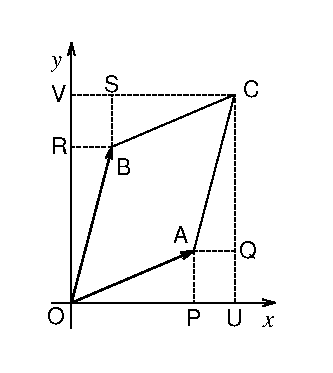
\includegraphics[width=4.5cm]{det2D2.eps}
    \caption{行列式の幾何学的意味の説明図\label{fig:det2D2}}
\end{figure}

さて, 点A, B, Cは図\ref{fig:det2D2}のように位置するとしよう。
点Cから$x$軸, $y$軸にそれぞれおろした垂線の足を点U, 点Vとし, 点Aから$x$軸, 点Bから$y$軸にそれぞれ
おろした垂線の足を点P, 点Rとする。点Aから直線CU, 点Bから直線CVにそれぞれおろした垂線の足を
点Q, 点Sとする。
明らかに, 三角形OAPと三角形CBSは合同であり, いずれも面積は$ac/2$である。
明らかに, 三角形OBRと三角形CAQは合同であり, いずれも面積は$bd/2$である。
明らかに, 長方形PAQUと長方形SBRVは合同であり, いずれも面積は$bc$である。
平行四辺形OACBは, 長方形OUCVからこれらの図形を取り去ったものだから, その面積は,
\begin{eqnarray*}
S&=&(a+b)(c+d)-2(ac/2)-2(bd/2)-2bc\\
 &=&ad-bc
\end{eqnarray*}
である。

上の結果は点A, B, Cの位置に若干の制限をつけて導いたが, この制限を
取り払うと, $ad-bc$の値がマイナスになることもある\footnote{例えば点Aと点Bの位置を
入れ替えてみると, 同じ議論で$S=bc-ad$になる。}。ただしそういう場合でも, 
$|ad-bc|$が$S$に等しいということは変わらずに正しい\footnote{$ad-bc$が
マイナスになるのは, ${\bf a}$から${\bf b}$に右ネジ\index{みぎねじ@右ネジ}をまわすときに, ネジの
進む方向が平面から下向き(君から遠ざかる方向)の場合である。}。

\begin{q}\label{q:matrix_triangle_area} ${\bf a}=(21, 8)$, ${\bf b}=(19, 9)$を
2辺とする三角形の面積を求めよ。注: これを, 高校数学でよく使う, 
$\sqrt{|{\bf a}|^2|{\bf b}|^2-({\bf a}\bullet{\bf b})^2}$
という公式で解こうとすると大変な計算になる。
\end{q}

\begin{faq}{\small\textgt{$S=|ad-bc|$を高校で教えないのはなぜでしょう?}
... 一部の高校や予備校では教えているようですが。}\end{faq}

\begin{q}\label{q:matrix_det_swap2D} 2次正方行列$A$の, 第1行と第2行を入れ替えて
できる行列を$A'$とする。次式を示せ\footnote{同様に, 列を入れ替えた行列の行列式も$-\det A$となる。}。
\begin{eqnarray}
\det A'=-\det A
\end{eqnarray}
\end{q}

\begin{q}\label{q:matrix_detAB_detBA_2D} 行列$A, B$を, 
\begin{eqnarray} 
A=\begin{bmatrix}
a & b \\
c & d \\
\end{bmatrix},\,\,\,\,
B=\begin{bmatrix}
p & q \\
r & s \\
\end{bmatrix}
\end{eqnarray}
とする。$\det A$, $\det B$, $\det (AB)$をそれぞれ計算して, 次式が成り立つことを確認せよ:
\begin{eqnarray}
\det (AB)=(\det A)(\det B)\label{eq:detABdetAdetB}
\end{eqnarray}
\end{q}\mv

このように, 一般的に, 行列の積の行列式は, 各行列の行列式の積に等しい(これは3次以上の
行列式についても成り立つことが証明できる)。

歴史的には, 行列式は, 行列そのものよりも早く発明(発見)された。また, 
行列式は英語でdeterminantというが, その中には行列(matrix)という語は入っていない。
そのことからもわかるように, 行列と行列式は(互いによく関連しているものの), 
それぞれ独立した数学的な対象だと考えるほうが適切かもしれない。

なお, 行列式の概念に世界で最初に到達したのは, 日本の和算家\footnote{日本の伝統的な数学を和算(わさん)という。}
である関孝和\index{せきたかかず@関孝和}だと言われている。
\vv



\section{逆行列}

さて, 行列の足し算や引き算, 掛け算はわかった。では割り算はどうだろう? 
行列では, 「割り算」を考えるかわりに, 「逆行列」というものを考える。

正方行列$A$について, ある行列$B$によって, 
\begin{eqnarray}
AB=BA=E\label{eq:def_invmatrix}
\end{eqnarray}
とできるとき, $B$を$A$の\underline{逆行列}(inverse matrix)\index{ぎゃくぎょうれつ@逆行列}と言って, 
$A^{-1}$とあらわす(定義)
\footnote{逆行列の定義式(\ref{eq:def_invmatrix})は, 
$AB=E$と$BA=E$という2つの条件を含んでいるが, 実は, このうち片方が成り立てば, もう片方は
自動的に成り立つことが知られている。その証明は大学の数学に譲る。}。

\begin{q}\label{q:matrix_inv2D} $\det A$が0でないような2次正方行列
\begin{eqnarray} A=\begin{bmatrix}
a & b \\
c & d \\
\end{bmatrix}\end{eqnarray}
について, 以下の行列は逆行列であることを確認せよ\footnote{3次以上の正方行列についても, 
これと同様の式が「余因子行列」\index{よいんしぎょうれつ@余因子行列}というもので構成できる。}。
\begin{eqnarray} \frac{1}{\det A}\begin{bmatrix}
d & -b \\
-c & a \\
\end{bmatrix}\label{eq:matrixinv}\end{eqnarray}
\end{q}\mv

この\eref{eq:matrixinv}は, $\det A$が0ならば分母が0になってしまうので, 
計算できない。従って, $\det A=0$ならば逆行列は存在しないのだ。逆行列は, いわば, 
普通の数における逆数のような立場の行列である。しかし, 普通の数ならば, 0
でない数ならどんな数でも逆数を持つが, 行列の場合は, たとえ$O$でなくても逆行列を
持たない行列がある。例えば, 以下の行列には, どんな行列を掛けても$E$にすることはできない(従って
逆行列を持たない)。
\begin{eqnarray} \begin{bmatrix}
1 & 0 \\
0 & 0 \\
\end{bmatrix}\end{eqnarray}

$\det A \neq 0$であるような正方行列, すなわち逆行列が存在するような行列を, 
\underline{正則行列} \index{せいそくぎょうれつ@正則行列} (regular matrix)という。

注: \eref{eq:matrixinv}を逆行列の定義であると思っている人がいるが, 
それはよくない。\eref{eq:matrixinv}は正方行列が2次のとき
にしか成り立たない。本来の\eref{eq:def_invmatrix}
を使う定義の方が, ずっとシンプルで一般性が高い。定義は
シンプルで一般的でなければならないのだ。


\begin{faq}{\small\textgt{逆行列の定義を問われて「$AB=BA=E$となるような行列」と答えたら不正解にされました。
なぜですか?}
... 省略しすぎですね。数学では, 出てくる変数や文字をきちんと定義しなければなりません。}\end{faq}

\begin{faq}{\small\textgt{でも,「正方行列$A, B$, 単位行列$E$について, $AB=BA=E$と
なるような行列」と答えたらまた不正解にされました。なぜですか?}
... 君の答案では$A, B, E, AB, BA$という5つの行列が出てきますが, そのうちの
どれが「逆行列」なのかはっきりしないからです。}\end{faq}

\begin{faq}{\small\textgt{でも,「正方行列$A, B$, 単位行列$E$について, $AB=BA=E$と
なるような$B$」と答えたらまた不正解にされました。なぜですか?}
... 逆行列は, 単体で成り立つ概念ではなく, 別の行列との関係で成り立つ概念です。
君の答案では, 「となるような$B$を\underline{$A$の}逆行列という」とまで答えれば
正解です。}\end{faq}

\begin{faq}{\small\textgt{なんか揚げ足取られている気がします。}
... 論理というのは緻密なものなのです。}\end{faq}

\begin{q}\label{q:matrix_AinvBinv2D} 次の行列について, 逆行列をそれぞれ求めよ。
\begin{eqnarray*}
A=\begin{bmatrix}
1 & 2 \\
-1 & 1 \\
\end{bmatrix}
,\,\,\,\, 
B=\begin{bmatrix}
2 & 0 \\
1 & 1 \\
\end{bmatrix}
\end{eqnarray*}
\end{q}\mv

\begin{q}\label{q:matrix_regular2D} $A$, $B$を任意の正則行列とする。
\begin{enumerate}
\item $AB$は正則行列であることを示せ。
\item 次式を示せ:
\begin{eqnarray}
(AB)^{-1}=B^{-1}A^{-1}
\end{eqnarray}
\end{enumerate}\end{q}
\mv

\begin{q}\label{q:matrix_det_inv2D} 2次の正則行列
$A$について, 次式が成り立つことを示せ:
\begin{eqnarray}
\det A^{-1}=\frac{1}{\det A}\label{q:matrix_det_inv}
\end{eqnarray}
\end{q}
\vv



\section{連立一次方程式}

例として, 二元連立一次方程式
\begin{eqnarray}\begin{cases}
2x+y=1\\
x+y=2
\end{cases}\end{eqnarray}
を考えよう。これは, 以下のように書くこともできる:
\begin{eqnarray}
\begin{bmatrix}
2 & 1 \\
1 & 1 \\
\end{bmatrix}
\begin{bmatrix}
x \\
y \\
\end{bmatrix}
=\begin{bmatrix}
1 \\
2 \\
\end{bmatrix}
\end{eqnarray}
この左辺の行列を$A$と書くと, \eref{eq:matrixinv}より, 
\begin{eqnarray*}
A^{-1}=\frac{1}{2\times 1 - 1 \times 1}
\begin{bmatrix}
1 & -1 \\
-1 & 2 \\
\end{bmatrix}
=\begin{bmatrix}
1 & -1 \\
-1 & 2 \\
\end{bmatrix}
\end{eqnarray*}
である。さて, 
\begin{eqnarray}
A\begin{bmatrix}
x \\
y \\
\end{bmatrix}
=\begin{bmatrix}
1 \\
2 \\
\end{bmatrix}
\end{eqnarray}
なので, この両辺に左から$A^{-1}$を掛けると, 
\begin{eqnarray}
A^{-1}A\begin{bmatrix}
x \\
y \\
\end{bmatrix}
=A^{-1}\begin{bmatrix}
1 \\
2 \\
\end{bmatrix}
\end{eqnarray}
となるが, $A^{-1}A=E$なので, 
\begin{eqnarray}
&&\begin{bmatrix}
x \\
y \\
\end{bmatrix}
=A^{-1}\begin{bmatrix}
1 \\
2 \\
\end{bmatrix}\nonumber\\
&&=\begin{bmatrix}
1 & -1 \\
-1 & 2 \\
\end{bmatrix}
\begin{bmatrix}
1 \\
2 \\
\end{bmatrix}
=\begin{bmatrix}
-1 \\
3 \\
\end{bmatrix}
\end{eqnarray}
となる(連立方程式が解けた!)。

一般に, 二元連立一次方程式は, 実数$a, b, c, d, p, q$を
使って以下のように書ける:
\begin{eqnarray}\begin{cases}
ax+by=p\\
cx+dy=q
\end{cases}\end{eqnarray}
これは, 
\begin{eqnarray}
A=\begin{bmatrix}
a & b \\
c & d \\
\end{bmatrix}
\end{eqnarray}
とすると, 以下のように書くことができる:
\begin{eqnarray}
A\begin{bmatrix}
x \\
y \\
\end{bmatrix}
=\begin{bmatrix}
p \\
q \\
\end{bmatrix}
\end{eqnarray}
もし$A$の逆行列$A^{-1}$が存在すれば, それを左から掛けて, 
\begin{eqnarray}
\begin{bmatrix}
x \\
y \\
\end{bmatrix}
=A^{-1}\begin{bmatrix}
p \\
q \\
\end{bmatrix}
\end{eqnarray}
と, 解くことができる。このように, 連立一次方程式\index{れんりついちじほうていしき@連立一次方程式}は, 行列とベクトルの掛け算で
書き表して, その係数で構成される行列(係数行列という。\index{けいすうぎょうれつ@係数行列}ここでは$A$)の逆行列
を求め, それを左から掛けることで, 解くことができる\footnote{無論, そんな
ことをしないで, 普通に変数をひとつずつ消していっても解けるのだが, 数学には
いろんなアプローチがあって, それぞれ長所や短所があるのだ。}。

ところが, 先に見たように, $A$の行列式$\det A$が0の場合は, 逆行列$A^{-1}$
は存在しない。そのような場合はどうなるのだろう? 例として以下の
方程式を考えよう:
\begin{eqnarray}\begin{cases}
x+2y=1\\
2x+4y=2
\end{cases}\label{eq:matrix_exmpl_2eq}\end{eqnarray}
これは次式と同じである:
\begin{eqnarray}
\begin{bmatrix}
1 & 2 \\
2 & 4 \\
\end{bmatrix}
\begin{bmatrix}
x \\
y \\
\end{bmatrix}
=\begin{bmatrix}
1 \\
2 \\
\end{bmatrix}
\end{eqnarray}
ところが, この係数行列$A$について, 
\begin{eqnarray*}\det A=1\times4-2\times2=0\end{eqnarray*}
だから, $A^{-1}$は定義できない。仕方ないからもとの方程式(\ref{eq:matrix_exmpl_2eq})
に戻って考えると, 第一式($x+2y=1$)を2倍したものが, 第二式($2x+4y=2$)と同じであることがわかる。
つまり, この連立方程式は, 本質的には1つの式:
\begin{eqnarray}
x+2y=1
\end{eqnarray}
に過ぎない。変数が2つあって, 式は1つだけなのだから, この
方程式は一意的には解けない。解は, 例えば$(x, y)=(1, 0)$とか
$(0, 1/2)$とか, 無数にたくさんある。こういうケースを, \underline{不定}
\index{ふてい@不定}という。

では, 次のような場合はどうだろう? 
\begin{eqnarray}\begin{cases}
x+2y=1\\
2x+4y=3
\end{cases}\end{eqnarray}
これも, 係数行列の行列式は0になる。この場合は, 「第一式$\times2-$第二式」
を考えると, 
\begin{eqnarray}
0=-1
\end{eqnarray}
となってしまう。これは絶対に成り立たない。$x, y$がどのような値をとろうが, 
成立させることができない方程式である。つまり, 解は存在しない。このような
ケースを, \underline{不能} \index{ふのう@不能}という。
\vv


\section{固有値と固有ベクトル}
\index{こゆうち@固有値}\index{こゆうべくとる@固有ベクトル}

正方行列$A$に対して, ある実数$\lambda$と, ある(${\bf 0}$でない)ベクトル${\bf x}$によって, 
\begin{eqnarray}
A{\bf x}=\lambda {\bf x}\label{eq:def_eigenvec}
\end{eqnarray}
となるとき, ${\bf x}$を$A$の\underline{固有ベクトル} (eigenvector)といい, 
$\lambda$を$A$の\underline{固有値} (eigenvalue)という(定義)。
これは, 行列の応用において, 非常に重要な概念である。\\

{\small 注: なぜか\eref{eq:def_eigenvec}を${\bf x}A={\bf x}\lambda$のように
書く人がいる。特殊な状況設定をすればこのように書くことも
無いではないのだが(それを今の段階で説明すると君は絶対に混乱する), 
そんなややこしいことをしないで, 素直に\eref{eq:def_eigenvec}の形で
覚えて欲しい。数と数の積ならどちらを先に書いてもかまわないのだが, 
行列やベクトルがからむ「積」は, 書き方や順序を不用意に
変えてはならないのだ。}

\begin{faq}{\small\textgt{固有ベクトルの定義で, なぜ${\bf x}$が${\bf 0}$でないという条件が
ついているのですか?}
... もし${\bf x}={\bf 0}$だと, $A$がどんな正方行列であろうが, また, $\lambda$
がどんなスカラーであろうが, $A{\bf x}=\lambda{\bf x}$が成り立っちゃうから
です。そういう「当たり前」の場合を, 固有ベクトルとはみなさない約束なのです。}\end{faq}

\begin{exmpl}\label{ex:matrix_eigen1} 以下の行列の固有値と固有ベクトルを求めてみよう:
\begin{eqnarray}
A=\begin{bmatrix}
5 & 3 \\
4 & 1 \\
\end{bmatrix}
\end{eqnarray}
固有値を$\lambda$, 固有ベクトルを${\bf x}$とすると, 定義から, $A{\bf x}=\lambda {\bf x}$が成り立つ。つまり, 
\begin{eqnarray}
A{\bf x}-\lambda {\bf x}={\bf 0}
\end{eqnarray}
である。ここで, $\lambda {\bf x}=\lambda E {\bf x}$と考えれば, 上の式は, 
\begin{eqnarray}
A{\bf x}-\lambda E{\bf x}={\bf 0}
\end{eqnarray}
すなわち, 
\begin{eqnarray}
(A-\lambda E){\bf x}={\bf 0}\label{eq:matrix_eigen_eq0}
\end{eqnarray}
となる。すなわち, 
\begin{eqnarray}
(A-\lambda E){\bf x}=
\begin{bmatrix}
5-\lambda & 3 \\
4          & 1-\lambda \\
\end{bmatrix}
\begin{bmatrix}
x \\
y \\
\end{bmatrix}
=\begin{bmatrix}
0 \\
0 \\
\end{bmatrix}\label{eq:matrix_eigen_eq000}
\end{eqnarray}
となる。さて, もしこの係数行列$A-\lambda E$に逆行列が存在すると仮定すれば, 
上の式の両辺に左から$(A-\lambda E)^{-1}$をかけて, 
\begin{eqnarray}
{\bf x}
=(A-\lambda E)^{-1}
\begin{bmatrix}
0 \\
0 \\
\end{bmatrix}
\end{eqnarray}
となる。$(A-\lambda E)^{-1}$がどんな行列であれ, この右辺は零ベクトル
になるしかない。すなわち, 
\begin{eqnarray}
{\bf x}
=\begin{bmatrix}
0 \\
0 \\
\end{bmatrix}={\bf 0}
\end{eqnarray}
となってしまう。これは, 固有ベクトルの定義に反している。従って, 
係数行列$A-\lambda E$に逆行列が存在してはならない\footnote{この論理は背理法である。}。従って, その行列式
は0にならねばならない。すなわち, 
\begin{eqnarray}
\det(A-\lambda E)=0\label{eq:matrix_tokusei}
\end{eqnarray}
である。\eref{eq:matrix_tokusei}を行列$A$の\underline{特性方程式} \index{とくせいほうていしき@特性方程式}
という(固有方程式ともいう\index{こゆうほうていしき@固有方程式})。これを解くと, 
\begin{eqnarray*}
&&(5-\lambda)(1-\lambda)-3\times4\\
&&=\lambda^2-6\lambda-7=(\lambda+1)(\lambda-7)=0
\end{eqnarray*}
となり, $\lambda=-1$と, $\lambda=7$となる。これで固有値が求まった。

では固有ベクトルを求めよう。まず, $\lambda=-1$のとき, 上の連立一次方程式(\ref{eq:matrix_eigen_eq000})は, 
\begin{eqnarray}
(A-\lambda E){\bf x}=
\begin{bmatrix}
6          & 3 \\
4          & 2 \\
\end{bmatrix}
\begin{bmatrix}
x \\
y \\
\end{bmatrix}
=\begin{bmatrix}
0 \\
0 \\
\end{bmatrix}\end{eqnarray}
となる。明らかに, この方程式は不定であり, これを満たす解は無数にあるが, 代表的に, 
\begin{eqnarray}
\begin{bmatrix}
x \\
y \\
\end{bmatrix}
=\begin{bmatrix}
1 \\
-2 \\
\end{bmatrix}
\end{eqnarray}
としよう。これが, 固有ベクトルのひとつである。

次に, $\lambda=7$のとき, 連立一次方程式(\ref{eq:matrix_eigen_eq0})は, 
\begin{eqnarray}
(A-\lambda E){\bf x}=
\begin{bmatrix}
-2         & 3 \\
4          & -6 \\
\end{bmatrix}
\begin{bmatrix}
x \\
y \\
\end{bmatrix}
=\begin{bmatrix}
0 \\
0 \\
\end{bmatrix}\end{eqnarray}
となる。この方程式も不定であり, これを満たす解は無数にあるが, 代表的に, 
\begin{eqnarray}
\begin{bmatrix}
x \\
y \\
\end{bmatrix}
=\begin{bmatrix}
3 \\
2 \\
\end{bmatrix}
\end{eqnarray}
としよう。これも, 固有ベクトルのひとつである。以上より, 行列$A$について, 
\begin{eqnarray*}\begin{cases}
\text{固有値が}-1\text{のとき, 固有ベクトル}
\begin{bmatrix}
1 \\
-2 \\
\end{bmatrix}\\
\\
\text{固有値が}7\text{のとき, 固有ベクトル}
\begin{bmatrix}
3 \\
2 \\
\end{bmatrix}
\end{cases}\end{eqnarray*}
である。
(例おわり)\end{exmpl}

このように, 固有値と固有ベクトルは, 互いに対になっている。一般に, 固有値・固有ベクトルの対
は, 高々, その行列の次数の数だけ存在する(中にはそれに足りない行列もあるが)。

注: 固有ベクトルは, ひとつに定まるものではない。実際, 固有ベクトルのスカラー倍も
固有ベクトルになるからだ(問\ref{q:matrix_eigen_scalar})。例えば, 上の例では, 

\begin{eqnarray*}\begin{cases}
\text{固有値が}-1\text{のとき, 固有ベクトル}
\begin{bmatrix}
-1 \\
2 \\
\end{bmatrix}\\
\\
\text{固有値が}7\text{のとき, 固有ベクトル}
\begin{bmatrix}
6 \\
4 \\
\end{bmatrix}
\end{cases}\end{eqnarray*}
と言っても構わない。

\begin{q}\label{q:matrix_eigen_scalar} 固有ベクトルをスカラー倍したもの(ただし0倍以外)
も, 固有ベクトルであることを示せ。ヒント: 固有ベクトルの定義に戻る!\end{q}

\begin{q}\label{q:matrix_eigen2D0} 以下の行列について, 固有値と固有ベクトルを求めよ。
\begin{eqnarray} \begin{bmatrix}
2 & 1\\
2 & 3\\
\end{bmatrix}\label{eq:matrix_lintrans_mondai}\end{eqnarray}
\end{q}

\begin{comment}
\begin{figure}[ht]
    \centering
    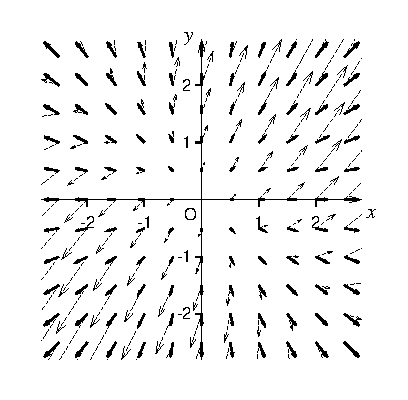
\includegraphics[width=8cm]{eigen.eps}
    \caption{\eref{eq:matrix_lintrans_mondai}の行列による線型変換のイメージ。
各点$(x, y)$にはベクトル$(x, y)$と(実線矢印), それを\eref{eq:matrix_lintrans_mondai}の行列
で線型変換したベクトル(点線矢印)が描かれている。2つの矢印が同方向に向いているとき(重なっているとき)
が固有ベクトルである。特に, 固有値が1のときの固有ベクトルは, もとの
ベクトルと, 向きも大きさも同じであることに注意しよう。}
\end{figure}
\mv
\end{comment}
\hv



\section{対角化}

先の例\ref{ex:matrix_eigen1}(P.\pageref{ex:matrix_eigen1})で, 
\begin{eqnarray}
A=\begin{bmatrix}
5 & 3 \\
4 & 1 \\
\end{bmatrix}\label{eq:matrixA_for_orthog}
\end{eqnarray}
という行列$A$について, 
\begin{eqnarray*}\begin{cases}
\text{固有値が}-1\text{のとき, 固有ベクトル}
\begin{bmatrix}
1 \\
-2 \\
\end{bmatrix}\\
\\
\text{固有値が}7\text{のとき, 固有ベクトル}
\begin{bmatrix}
3 \\
2 \\
\end{bmatrix}
\end{cases}\end{eqnarray*}
であることが示された。すなわち, 
\begin{eqnarray}\begin{cases}
\begin{bmatrix}
5 & 3 \\
4 & 1 \\
\end{bmatrix}
\begin{bmatrix}
1 \\
-2 \\
\end{bmatrix}
=-1\times\begin{bmatrix}
1 \\
-2 \\
\end{bmatrix}\\
\\
\begin{bmatrix}
5 & 3 \\
4 & 1 \\
\end{bmatrix}
\begin{bmatrix}
3 \\
2 \\
\end{bmatrix}
=7\times\begin{bmatrix}
3 \\
2 \\
\end{bmatrix}
\end{cases}\end{eqnarray}
である。これらをひとまとめにすると, 
\begin{eqnarray*}
\begin{bmatrix}
5 & 3 \\
4 & 1 \\
\end{bmatrix}
\begin{bmatrix}
1 & 3\\
-2 & 2\\
\end{bmatrix}
=\begin{bmatrix}
1 & 3\\
-2 & 2\\
\end{bmatrix}
\begin{bmatrix}
-1 & 0 \\
0 & 7 \\
\end{bmatrix}
\end{eqnarray*}
とできる\footnote{固有ベクトルの並べ順を左右入れ替えて, 
\begin{eqnarray*}
\begin{bmatrix}
5 & 3 \\
4 & 1 \\
\end{bmatrix}
\begin{bmatrix}
3 & 1\\
2 & -2\\
\end{bmatrix}
=\begin{bmatrix}
3 & 1\\
2 & -2\\
\end{bmatrix}
\begin{bmatrix}
7 & 0 \\
0 & -1 \\
\end{bmatrix}
\end{eqnarray*}
としてもよい。その場合, \eref{eq:matrix_orthogonalize_9}に相当する式は, 
\begin{eqnarray*}
Q=\begin{bmatrix}
3 & 1\\
2 & -2\\
\end{bmatrix}
\text{として, }\,\,\,
Q^{-1}AQ
=\begin{bmatrix}
7 & 0 \\
0 & -1 \\
\end{bmatrix}
\end{eqnarray*}
}。すると, 
\begin{eqnarray}
\begin{bmatrix}
1 & 3\\
-2 & 2\\
\end{bmatrix}^{-1}
\begin{bmatrix}
5 & 3 \\
4 & 1 \\
\end{bmatrix}
\begin{bmatrix}
1 & 3\\
-2 & 2\\
\end{bmatrix}
=\begin{bmatrix}
-1 & 0 \\
0 & 7 \\
\end{bmatrix}\label{eq:matrix_orthogonalize_6}
\end{eqnarray}
となることがわかる。ここで, 2つの固有ベクトルを列ベクトルとして並べてできる行列を$P$とする。つまり, 
\begin{eqnarray}
P=\begin{bmatrix}
1 & 3\\
-2 & 2\\
\end{bmatrix}
\end{eqnarray}
とすると, \eref{eq:matrix_orthogonalize_6}は, 
\begin{eqnarray}
P^{-1}AP
=\begin{bmatrix}
-1 & 0 \\
0 & 7 \\
\end{bmatrix}\label{eq:matrix_orthogonalize_9}
\end{eqnarray}
である。このように, 与えられた行列(ここでは$A$)に対して, ある行列$P$によって, $P^{-1}AP$
とすることで, 非対角成分が0の行列(そのような行列を対角行列\index{たいかくぎょうれつ@対角行列}という)
にすることを, \underline{対角化}\index{たいかくか@対角化}という。上の説明でわかるように, 
ある行列$A$を対角化するには, 次のような手順をとる:
\begin{itemize}
\item $A$の特性方程式を立てる。
\item それを解いて, $A$の固有値を求める。
\item 各固有値に対応する固有ベクトルを求める。
\item $A$の固有ベクトルを列ベクトルとして並べてできる行列を$P$とおく(慣習的には, 固有値の大きい順に)。
\item すると, $P^{-1}AP$は対角行列になる。その対角行列の対角成分(行番号と列番号が同じ成分)には, $A$の固有値が並ぶ。
\end{itemize}
\mv

注意: 行列$A$を対角化するための行列$P$は, ひとつに定まるものではない。

\begin{q}\label{q:matrix_orth2D_Pvariable} \eref{eq:matrixA_for_orthog}と, 
以下のそれぞれの$P$について, $P^{-1}AP$を計算せよ。
\begin{eqnarray*}
&&\text{(1)}\quad 
P=\begin{bmatrix}
1 & 3 \\
-2 & 2 \\
\end{bmatrix}\quad\quad 
\text{(2)}\quad 
P=\begin{bmatrix}
3 & 1 \\
2 & -2 \\
\end{bmatrix}\\
&&\text{(3)}\quad 
P=\begin{bmatrix}
-1 & 6 \\
2  & 4 \\
\end{bmatrix}
\end{eqnarray*}
\end{q}

\begin{q}\label{q:matrix_orth2D0} 以下の行列を対角化せよ:
\begin{eqnarray} \begin{bmatrix}
-1 & 2\\
-6 & 6\\
\end{bmatrix}\end{eqnarray}
\end{q}\mv

さて, ある2次正方行列$A$が, 行列$P$によって対角化されるとき, 
\begin{eqnarray}
P^{-1}AP
=\begin{bmatrix}
\lambda_1 & 0 \\
0 & \lambda_2 \\
\end{bmatrix}
\end{eqnarray}
となる($\lambda_1$と$\lambda_2$は$A$の固有値である)。両辺に, 左から$P$を, 右から$P^{-1}$を
それぞれ掛けると, 
\begin{eqnarray}
A
=P\begin{bmatrix}
\lambda_1 & 0 \\
0 & \lambda_2 \\
\end{bmatrix}P^{-1}
\end{eqnarray}
となる。従って, $A$の行列式は, 
\begin{eqnarray}
&&\det A\nonumber\\
&&=\det\Bigl(P\begin{bmatrix}
\lambda_1 & 0 \\
0 & \lambda_2 \\
\end{bmatrix}P^{-1}\Bigr)
=\det P\det\begin{bmatrix}
\lambda_1 & 0 \\
0 & \lambda_2 \\
\end{bmatrix}\det P^{-1}\nonumber\\
&&=\det P\det P^{-1}\det\begin{bmatrix}
\lambda_1 & 0 \\
0 & \lambda_2 \\
\end{bmatrix}=\det\begin{bmatrix}
\lambda_1 & 0 \\
0 & \lambda_2 \\
\end{bmatrix}\nonumber\\
&&=\lambda_1\lambda_2
\end{eqnarray}
となる(ここで\eref{eq:detABdetAdetB}, \eref{q:matrix_det_inv}を使った)。
つまり, 行列式は, 固有値の積に等しい (定理)。
\mv

対角化はいろんなことに応用できる。以下の例を考えよう:

\begin{exmpl}ある国の森林100$\,\,$km$^2$が山火事で荒廃して裸地・森林のモザイク状になった。その後を1年間調査した結果, 次のようなことがわかった:
1) 調査した裸地のうち, 8割は裸地のままで, 2割は植生が繁って森林になった
{\small (1年間でそんなに早く森林が回復するわけがない! というツッコミは勘弁してほしい)}。
2) 調査した森林のうち, 1割が再び山火事によって裸地になり, 9割は森林のままだった。
このような変化がずっと続くと仮定しよう。$n$年後の裸地(bare)・森林(forest)
のそれぞれの面積を$b_n$~km$^2$, $f_n$~km$^2$とすると, 
\begin{eqnarray}
\begin{bmatrix}
b_{n+1}\\
f_{n+1}\\
\end{bmatrix}=
\begin{bmatrix}
0.8 & 0.1\\
0.2 & 0.9\\
\end{bmatrix}
\begin{bmatrix}
b_n\\
f_n\\
\end{bmatrix}\label{eq:matrix_Markov3}
\end{eqnarray}
と書ける。$^\text{t}(b_n, f_n)$を${\bf c}_n$とおき, 上の式の右辺の係数行列を$A$とすれば, 
\eref{eq:matrix_Markov3}は次式のように書ける:
\begin{eqnarray} 
{\bf c}_{n+1}=A{~}{\bf c}_n
\end{eqnarray}
\end{exmpl}

\begin{q}\label{q:mtrix_exm_mMrkov} 
\begin{enumerate}
\item この行列$A$を対角化せよ。
\item ${\bf c}_n=A^n{~}{\bf c}_0$となることを示せ(${\bf c}_0$は現在の状態)。
\item 対角化の結果を用いて, $A^n$を計算せよ。(ヒント:$(P^{-1}AP)^n=P^{-1}A^nP$)
\item 現状で裸地が80$\,\,$km$^2$, 森林が20$\,\,$km$^2$とする。3年後のそれぞれの面積を予想せよ。
\item 長い将来($n \rightarrow \infty$), 森林と裸地はそれぞれどのくらいの面積になると予想されるか?
\end{enumerate}
\end{q}

このように, 時間的に変化する現象を, 複数の状態(上では森林と裸地)の混在として表現し, 
さらにその比率が, その瞬間の比率に依存して変化していくとみなす考え方を, 「マルコフ過程」\index{まるこふかて
い@マルコフ過程}という。上の話に草原と農地を含めて拡張したければ, 
ベクトル${\bf c}_n$を4次元の数ベクトルとし, 
係数行列$A$ (マルコフ過程の遷移行列\index{せんいぎょうれつ@遷移行列}と呼ばれる)
を4次の正方行列にすればよい。
\mv

\begin{faq}{\small\textgt{行列って何の役に立つのですか?} 
... むっちゃ役立ちます。例えば問\ref{q:mtrix_exm_mMrkov}のマルコフ過程は, 
生態学, 市場予測(経済学), 気象予測, 作物収穫予測などで使われます。
2次正方行列よりももっと大きな行列にも同様の理論が成り立ち, 
それは, 多くの変数が関与する統計学(多変量解析学)や, 電子や
原子の状態を解析する量子力学・量子化学, ものの強度や変形を解析する
材料力学・構造力学等, 多分野で中心的な役割をする理論です(特に対称行列と直交行列)。}\end{faq}
\hv

\section{3次の行列式}\label{sec:2Ddet}

これまで, 主に2次の正方行列について学んできた。初学者が行列に慣れたり基本的な概念を学ぶには, 
まず小さい行列でやる方が(取り扱いが簡単なので)よいからだ。しかし, 実際は, もっと大きな行列を
扱うことの方が多い。

既に学んだように, 2次正方行列
\begin{eqnarray}
A=\begin{bmatrix}a_1 & b_1\\
a_2 & b_2\\
\end{bmatrix}
\end{eqnarray}
の行列式\index{ぎょうれつしき@行列式}$\det (A)$は, $a_1b_2-a_2b_1$で定義される。この計算過程を図式的に書くと, 
図\ref{fig:Sarrus2D}のように, 左上から右下への2つの数字の積(図\ref{fig:Sarrus2D}の左; 
つまり$a_1b_2$)に正符号, 右上から左下への2つの数字の積(図\ref{fig:Sarrus2D}の右; 
つまり$a_2b_1$)に負符号をつけて, 足し合わせたものだ。要するに「左上×右下$-$
右上×左下」である。この操作を「たすきがけ」\footnote{本来は, 和服の袖をたくし
上げるために, 左肩から右脇, 右肩から左脇にかけて紐でしばること。}という。
\begin{figure}[h]
    \centering
    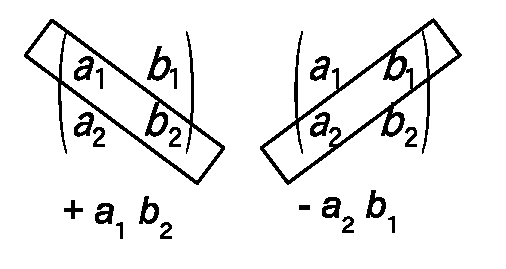
\includegraphics[width=4cm]{Sarrus2D.eps}
    \caption{2次の行列式(たすきがけ)}\label{fig:Sarrus2D}    
\end{figure}

この考え方を拡張して, 3次正方行列
\begin{eqnarray}
B=\begin{bmatrix}a_1 & b_1 & c_1\\
a_2 & b_2 & c_2\\
a_3 & b_3 & c_3\\
\end{bmatrix}\label{eq:univ_matrix_B}
\end{eqnarray}
の行列式$\det (B)$を, 次のように定義する: 図\ref{fig:Sarrus}上段の
ように, 「左上から右下への3つの数字の積」として, $a_1b_2c_3$, $a_2b_3c_1$, 
$a_3b_1c_2$を考え, これらに正符号をつける。一方, 図\ref{fig:Sarrus}下段の
ように, 「右上から左下への3つの数字の積」として, $a_3b_2c_1$, $a_2b_1c_3$, 
$a_1b_3c_2$を考え, これらに負符号をつける。そうしてこれらを足し合わせるのだ。
つまり, 
\begin{equation}\begin{split}
\det(B)&&:=a_1b_2c_3+a_2b_3c_1+a_3b_1c_2\\
       &&-a_3b_2c_1-a_2b_1c_3-a_1b_3c_2
\end{split}\label{eq:univ_matrix_Sarrus}\end{equation}
と定義する。これを\underline{サラスの公式} \index{さらすのこうしき@サラスの公式}と呼ぶ。
\begin{figure}[h]
    \centering
    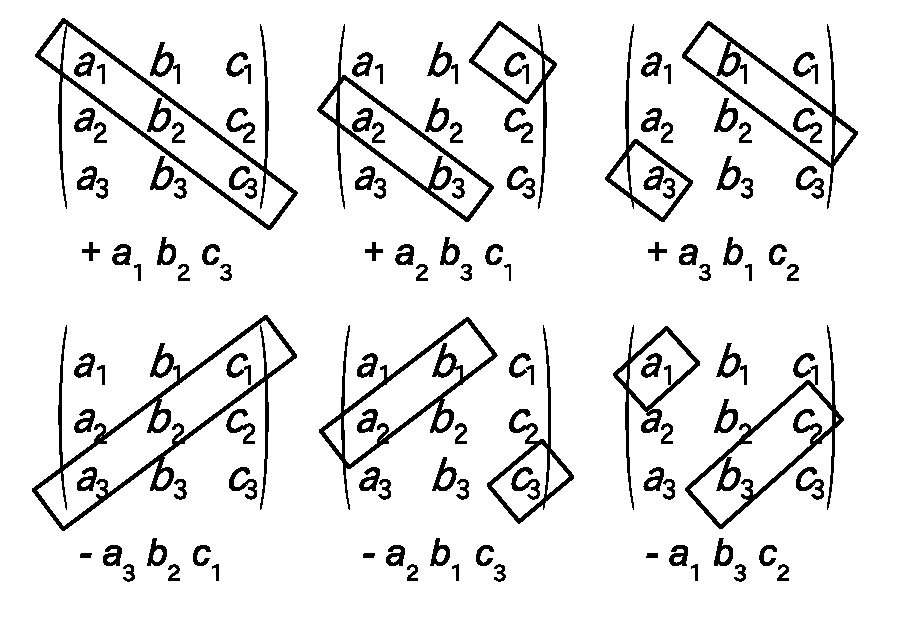
\includegraphics[width=7cm]{Sarrus.eps}
    \caption{3次の行列式(サラスの公式)}\label{fig:Sarrus}
\end{figure}
\mv

\begin{q}\label{q:univ_det3D0} 以下の行列の行列式を計算せよ:
\begin{edaenumerate}
\item
\begin{eqnarray*} \begin{bmatrix}1 & 0 & 1\\
2 & 1 & 0\\
1 & -1 & 3\\
\end{bmatrix}\end{eqnarray*}
\item
\begin{eqnarray*} \begin{bmatrix}1 & 1 & 2\\
1 & 2 & 4\\
1 & 3 & 5\\
\end{bmatrix}\end{eqnarray*}
\item
\begin{eqnarray*} \begin{bmatrix}1 & 2 & 2\\
1 & 4 & 4\\
1 & 6 & 5\\
\end{bmatrix}\end{eqnarray*}
\item
\begin{eqnarray*} \begin{bmatrix}1 & 2 & 1\\
2 & 4 & 0\\
3 & 6 & -1\\
\end{bmatrix}\end{eqnarray*}
\item
\begin{eqnarray*} \begin{bmatrix}1 & 2 & -1\\
-1 & 3 & -1\\
1 & 1 & 2\\
\end{bmatrix}\end{eqnarray*}
\item
\begin{eqnarray*} \begin{bmatrix}2 & 1 & -1\\
3 & -1 & -1\\
1 & 1 & 2\\
\end{bmatrix}\end{eqnarray*}
\item
\begin{eqnarray*} \begin{bmatrix}-1 & 3 & -1\\
1 & 1 & 2\\
1 & 2 & -1\\
\end{bmatrix}\end{eqnarray*}
\end{edaenumerate}\end{q}
\mv



\section{ベクトルの線型変換}

行列の乗算のルールで, 2次元の列ベクトルに, 左から2次正方行列を掛けると, 結果は, 2次元の列ベクトルになる。例えば, 
\begin{eqnarray}
A=\begin{bmatrix}
1 & 2 \\
0 & 1 \\
\end{bmatrix}
,\,\,\,\, 
{\bf x}=\begin{bmatrix}
2 \\
3 \\
\end{bmatrix}
\end{eqnarray}
とすれば, 
\begin{eqnarray*}
A{\bf x}=\begin{bmatrix}
1 & 2 \\
0 & 1 \\
\end{bmatrix}
\begin{bmatrix}
2 \\
3 \\
\end{bmatrix}
=\begin{bmatrix}
1\times2 + 2\times3 \\
0\times2 + 1\times3 \\
\end{bmatrix}
=\begin{bmatrix}
8 \\
3 \\
\end{bmatrix}
\end{eqnarray*}
となる。このような操作は, 列ベクトルを別の列ベクトルに変換する操作であると
みなすことができる。そこで, このように, 列ベクトルに正方行列を左から
掛けることで別の列ベクトルにする操作のことを, \underline{線型変換} \index{せんけいへんかん@線型変換}
(linear transformation)とか\underline{一次変換} \index{いちじへんかん@一次変換}と呼ぶ
\footnote{大学数学では, 線型変換をもっと一般的・抽象的に定義し直す。}。

さて, 列ベクトルを, 平面上の位置ベクトルとみなせば, 列ベクトルの線型変換は, 
平面上の点を移動させることに相当する。例えば, 
\begin{eqnarray}
A=\begin{bmatrix}
-1 & 0 \\
0 & 1 \\
\end{bmatrix}
\end{eqnarray}
とすれば, 行列$A$による線型変換は, 点$(x, y)$を, 
\begin{eqnarray}
\begin{bmatrix}
-1 & 0 \\
0 & 1 \\
\end{bmatrix}
\begin{bmatrix}
x \\
y \\
\end{bmatrix}
=\begin{bmatrix}
-x \\
y \\
\end{bmatrix}
\end{eqnarray}
というふうに, 点$(-x, y)$に移すことがわかる。これは, $x$座標の正負を逆転
するという操作であり, つまり, $y$軸に関する対称移動である。

\begin{q}\label{q:matrix_lintrans2D0} 以下の行列であらわされる線型変換は, 平面上の点をどのように移すか? 
\begin{edaenumerate}<3>
\item 
\begin{eqnarray*} \begin{bmatrix}
1 & 0 \\
0 & 1 \\
\end{bmatrix}\end{eqnarray*}
\mv
\item 
\begin{eqnarray*} \begin{bmatrix}
1 & 0 \\
0 & -1 \\
\end{bmatrix}\end{eqnarray*}
\mv
\item 
\begin{eqnarray*} \begin{bmatrix}
-1 & 0 \\
0 & -1 \\
\end{bmatrix}\end{eqnarray*}
\mv
\item 
\begin{eqnarray*} \begin{bmatrix}
0 & 1 \\
1 & 0 \\
\end{bmatrix}\end{eqnarray*}
\mv
%\item 
%\begin{eqnarray*} \begin{bmatrix}
%2 & 0 \\
%0 & 2 \\
%\end{bmatrix}\end{eqnarray*}
%\mv
\item 
\begin{eqnarray*} \begin{bmatrix}
2 & 0 \\
0 & 1 \\
\end{bmatrix}\end{eqnarray*}
\mv
\item 
\begin{eqnarray*} \begin{bmatrix}
1 & 0 \\
0 & 0 \\
\end{bmatrix}\end{eqnarray*}
\end{edaenumerate}\end{q}
\mv

\begin{q}\label{q:matrix_lintrans2D2} 前問の, (2), (3), (4)の行列は, いずれも, 2乗したら
単位行列になる。なぜだろうか? 平面上の線型変換という観点から考察せよ。\end{q}
\mv

次に, 平面上の点を回転\index{かいてん@回転}するような変換を考えてみよう。
極座標(\pref{eq:2Dpolar})を考えると, ある点Pの座標(位置ベクトル)は, 
\begin{eqnarray}
\begin{bmatrix}
x \\
y \\
\end{bmatrix}=
\begin{bmatrix}
r \cos \theta \\
r \sin \theta \\
\end{bmatrix}
\end{eqnarray}
と表現できる。ここで$r$は原点OからPまでの距離であり, $\theta$は$x$軸からOPまでの角度(左回り)
である。さて, この点を, 左に$\alpha$だけ回転すると, 当然ながら, その座標は, 
\begin{eqnarray}
\begin{bmatrix}
r \cos (\theta+\alpha) \\
r \sin (\theta+\alpha) \\
\end{bmatrix}
\end{eqnarray}
となる。加法定理(\pref{eq:add_sin1})を使ってこれを変形すれば, 
\begin{eqnarray*}
\begin{bmatrix}
r \cos \theta \cos \alpha - r \sin \theta \sin \alpha\\
r \sin \theta \cos \alpha + r \cos \theta \sin \alpha\\
\end{bmatrix}=
\begin{bmatrix}
x \cos \alpha - y \sin \alpha\\
y \cos \alpha + x \sin \alpha\\
\end{bmatrix}\\
=\begin{bmatrix}
\cos \alpha & -\sin \alpha\\
\sin \alpha & \cos \alpha\\
\end{bmatrix}
\begin{bmatrix}
x\\
y\\
\end{bmatrix}
\end{eqnarray*}
となる。すなわち, 以下の行列:
\begin{eqnarray}
\begin{bmatrix}
\cos \alpha & -\sin \alpha\\
\sin \alpha & \cos \alpha\\
\end{bmatrix}\label{eq:2Drotmatrix}
\end{eqnarray}
が, 「回転という線型変換」を表す行列である。

\begin{faq}{\small\textgt{回転の行列をなかなか覚えられません。どこがcosでどこがsinでどこにマイナスがつくのかとか。}
... \eref{eq:2Drotmatrix}ですね。記憶に自信がないときは, 
試しに$\alpha=0$を代入してみると良いのです。角度0の回転とは,
 何もしないことですから, そのときこの行列は単位行列になるはずです
(実際, そうなるでしょ?)。sinとcosを間違えてたら, 一発でわかります。}\end{faq}

\begin{q}\label{q:matrix_lintrans2D4} 以下のような, 座標平面上の点の移動を表す行列を, それぞれ求めよ:
\begin{enumerate}
\item $x$軸に関して対称移動。
\item 原点に関して対称移動。
\item 原点を中心として, 角$\pi/4$だけ左回りに回転。
\end{enumerate}\end{q}
\mv

\begin{q}\label{q:matrix_lintrans2D6} \eref{eq:2Drotmatrix}の行列を$A$とする。以下を求めよ:\\
(1) $\det A$  (2) $A^{-1}$  (3) $A^2$\end{q}
\mv

\begin{exq}\label{q:univ_det3D3} \eref{eq:univ_matrix_B}の行列式を考える。
\begin{eqnarray*}
{\bf a}=\begin{bmatrix}a_1\\
a_2\\
a_3\\
\end{bmatrix},\,\,
{\bf b}=\begin{bmatrix}b_1\\
b_2\\
b_3\\
\end{bmatrix}
,\,\,
{\bf c}=\begin{bmatrix}c_1\\
c_2\\
c_3\\
\end{bmatrix}
\end{eqnarray*}
とする。
\begin{enumerate}
\item 
\begin{eqnarray}
({\bf a}\times{\bf b})\bullet{\bf c}\label{eq:scalar3product00}
\end{eqnarray}
は, $\det(B)$に一致することを示せ。
\item このことを利用して, $|\det (B)|$は, ${\bf a}$, ${\bf b}$, ${\bf c}$が張る平行六面体(互いに平行な菱型3組からできる立体。豆腐を斜めにひしゃげたような形)の体積に等しいことを示せ。
\item ${\bf a}={\bf b}$または${\bf a}={\bf c}$または${\bf b}={\bf c}$のとき, $\det(B)=0$であることを示せ(ヒント: 計算しないでも示せる!)
\end{enumerate}
この性質は, 2次の行列式が「平行四辺形の面積」を表すことの拡張版だ, ということに気づいただろうか? このように, 行列式は, 面積や体積のようなものを表すのだ。このことは, いずれ, 複数の変数による積分(面積分や体積分)で使う。1変数による積分について学んだ「置換積分」が, 面積分や体積分では, 行列式を使って表されるのである(ヤコビアンという。興味のある人は調べてみよ)。
\end{exq}

\begin{exq}\label{q:univ_det3D2} 3次正方行列$B$について, 
\begin{enumerate}
\item 第1列と第2列を入れ替えてできる行列を$B'$とする。
\begin{eqnarray}\det B'=-\det B\end{eqnarray}
であることを示せ。
\item 第1列と第3列の入れ替えや, 第2列と第3列の入れ替えでも, 行列式は符合が逆転することを示せ。
\item 同様のことが行についても成り立つことを示せ。すなわち, 行列$B$の任意の2つの列を入れ替えてできる行列の行列式は符合が逆転することを示せ。
\end{enumerate}
 このような, 列の入れ替え(又は行の入れ替え)によって符合が逆転する, というのは, 2次や3次だけでなく, もっと大きな行列式にも成り立つ。いわば, 行列式の本質的な性質(のひとつ)である。このことは, 化学において, 分子内の電子の挙動を表現するときに使われる。それがなぜなのかは, 今はわからなくてよい。電子は行列式と相性が良い, ということは頭の片隅に置いておこう。勉強を続けていれば, そのうち, 「ああ, こういうことだったのか!」と, わかるときが来るだろう。
\end{exq}


\section*{問題の解答}

% 以下の行列$A, B, C$について, 問いに答えよ。
\noindent{\textbf{答}}\ref{q:matrix_basic0}  
\begin{eqnarray*}
(1)\,\,\,\,&&2A=
\begin{bmatrix}
2 & 4 \\
-2 & 2 \\
\end{bmatrix}
,\,\,
A-B=
\begin{bmatrix}
-1 & 2 \\
-2 & 0 \\
\end{bmatrix}\\
(2)\,\,\,\,&&AB=
\begin{bmatrix}
4 & 2 \\
-1 & 1 \\
\end{bmatrix}
,\,\,
BA=
\begin{bmatrix}
2 & 4 \\
0 & 3 \\
\end{bmatrix}\\
&&\text{従って, $AB\ne BA$。}\\
(3)\,\,\,\,&&(AB)C=
\begin{bmatrix}
4 & 2 \\
-1 & 1 \\
\end{bmatrix}
\begin{bmatrix}
3 & 1 \\
1 & -2 \\
\end{bmatrix}
=
\begin{bmatrix}
14 & 0 \\
-2 & -3 \\
\end{bmatrix}
, \\
&&A(BC)=
\begin{bmatrix}
1 & 2 \\
-1 & 1 \\
\end{bmatrix}
\begin{bmatrix}
6 & 2 \\
4 & -1 \\
\end{bmatrix}
=\begin{bmatrix}
14 & 0 \\
-2 & -3 \\
\end{bmatrix}\\
&&\text{従って, }(AB)C=A(BC)\\
(4)\,\,\,\,&&A(B+C)=
\begin{bmatrix}
1 & 2 \\
-1 & 1 \\
\end{bmatrix}
\begin{bmatrix}
5 & 1 \\
2 & -1 \\
\end{bmatrix}
=\begin{bmatrix}
9 & -1 \\
-3 & -2 \\
\end{bmatrix}
, \\
&&AB+AC=
\begin{bmatrix}
4 & 2 \\
-1 & 1 \\
\end{bmatrix}
+\begin{bmatrix}
5 & -3 \\
-2 & -3 \\
\end{bmatrix}
=\begin{bmatrix}
9 & -1 \\
-3 & -2 \\
\end{bmatrix}\\
&&\text{従って, }A(B+C)=AB+AC
\end{eqnarray*}
\mv

%\noindent{\textbf{答}}\ref{q:matrix_basic01}  略。

%\noindent{\textbf{答}}\ref{q:matrix_unit0}  略(各自計算せよ)。\mv

%
\noindent{\textbf{答}}\ref{q:matrix_det2D} 
$\det A=1\times1-2\times(-1)=3$。
$\det B=2\times1-0\times1=2$。
\mv

%
\noindent{\textbf{答}}\ref{q:matrix_detunit2D}  $\det E =1$
\mv

%
\noindent{\textbf{答}}\ref{q:matrix_det_difference} 
両者は全く違う。行列は, 数を格子状に並べたもの。行列を構成する
個々の数を行列の成分という。行列式は行列の成分に関する, ある種の多項式。
\mv

%
\noindent{\textbf{答}}\ref{q:matrix_triangle_area} 
$\bf a$と$\bf b$で張られる平行四辺形の面積は, 
\begin{eqnarray*}\det
\begin{bmatrix}
21 & 19 \\
8 & 9 \\
\end{bmatrix}
=21\times9-19\times8=37\end{eqnarray*}
この平行四辺形の半分が${\bf a}$と${\bf b}$を2辺とする三角形だから, 
この三角形の面積は, $37/2$
\mv

%
\noindent{\textbf{答}}\ref{q:matrix_det_swap2D}  行列$A$を
\begin{eqnarray*}A=\begin{bmatrix}
a & b \\
c & d \\
\end{bmatrix}\end{eqnarray*}
とすると, $\det A=ad-bc$。一方, $A$の第1行と第2行を入れ替えた行列$A'$は次のようになる, 
\begin{eqnarray*}A'=\begin{bmatrix}
c & d \\
a & b \\
\end{bmatrix}\end{eqnarray*}
この行列式は, $\det A'=cb-da=-(ad-bc)$となる。これは$-\det A$に等しい。
\mv

%
\noindent{\textbf{答}}\ref{q:matrix_detAB_detBA_2D}
\begin{eqnarray*}
\det (AB)&=&
\det
\begin{bmatrix}
ap+br & aq+bs \\
cp+dr & cq+ds \\
\end{bmatrix}
\\
&=&(ap+br)(cq+ds)-(aq+bs)(cp+dr)\\
&=&acpq+adps+bcqr+bdrs\\
&-&(acpq+adqr+bcps+bdrs)\\
&=&adps+bcqr-adqr-bcps
\end{eqnarray*}
\begin{eqnarray*}
(\det A)(\det B)&=&(ad-bc)(ps-qr)\\
&=&adps+bcqr-adqr-bcps
\end{eqnarray*}
従って, $\det (AB)=(\det A)(\det B)$
\mv

%
%2011.07.27 ヤマサキ解答追加。
\noindent{\textbf{答}}\ref{q:matrix_inv2D}
\eref{eq:matrixinv}の行列を$B$と置く。
\begin{eqnarray*}
AB &=& 
\begin{bmatrix}
a & b \\
c & d \\
\end{bmatrix}
 \frac{1}{\text{det}A} 
\begin{bmatrix}
d & -b \\
-c & a \\
\end{bmatrix}
 \\
&=&  \frac{1}{\text{det}A} 
\begin{bmatrix}
a & b \\
c & d \\
\end{bmatrix}
\begin{bmatrix}
d & -b \\
-c & a \\
\end{bmatrix}
 \\
&=& \frac{1}{\text{det}A} 
\begin{bmatrix}
ad-bc & ab-ab \\
cd-cd & ad-bc \\
\end{bmatrix}
 \\
&=& \frac{1}{\text{det}A} 
\begin{bmatrix}
\text{det}A & 0 \\
0 & \text{det}A \\
\end{bmatrix}
 =  
\begin{bmatrix}
1 & 0 \\
0 & 1 \\
\end{bmatrix}
 = E
\end{eqnarray*}
($BA=E$となることはここでは省略。各自, 確かめよ) 
従って, 定義より, 行列$B$は$A$の逆行列である。
\mv

%
\noindent{\textbf{答}}\ref{q:matrix_AinvBinv2D} 
\begin{eqnarray*}
A^{-1}=
\begin{bmatrix}
1/3 & -2/3 \\
1/3 & 1/3 \\
\end{bmatrix}
,\,\,
B^{-1}=
\begin{bmatrix}
1/2 & 0 \\
-1/2 & 1 \\
\end{bmatrix}
\end{eqnarray*}
\mv

%
\noindent{\textbf{答}}\ref{q:matrix_regular2D}  
\begin{enumerate}
\item 式(\ref{eq:detABdetAdetB})より, $\det (AB) =(\det A)(\det B)$。
ここで, $A, B$はともに正則行列なので, $\det A\ne0$かつ$\det B\ne0$である。
従って, $(\det A)(\det B)\ne0$。従って, $\det (AB)\ne0$。従って, $AB$は正則行列。
\item $(AB)(B^{-1}A^{-1})=A(BB^{-1})A^{-1}=AEA^{-1}$\\$=AA^{-1}=E$。
従って, $B^{-1}A^{-1}$は$AB$の逆行列である。
\end{enumerate}
\mv

%
\noindent{\textbf{答}}\ref{q:matrix_det_inv2D}  $AA^{-1}=E$だから, 
$\det AA^{-1}=\det E=1$である。一方,  
$\det AA^{-1}=(\det A)(\det A^{-1})$。これらの2つの式を
組み合わせると, $(\det A)(\det A^{-1})=1$。この両辺を$\det A$
で割ると, $\det A^{-1}=1/\det A$。
\mv


% 固有値と固有ベクトル
% 
\noindent{\textbf{答}}\ref{q:matrix_eigen2D0}  この行列を$A$とすると, 
その特性方程式は, \eref{eq:matrix_tokusei}より, 
\begin{eqnarray*}
&&\det(A-\lambda E)=(2-\lambda)(3-\lambda)-1\times2\\
&&=\lambda^2-5\lambda+4=(\lambda-1)(\lambda-4)=0
\end{eqnarray*}
となる。これを満たすのは, $\lambda=1$と, $\lambda=4$である。
これが固有値である。では固有ベクトルを求めよう。まず, $\lambda=1$のとき, 
\begin{eqnarray}
(A-\lambda E){\bf x}=
\begin{bmatrix}
1          & 1 \\
2          & 2 \\
\end{bmatrix}
\begin{bmatrix}
x \\
y \\
\end{bmatrix}
=\begin{bmatrix}
0 \\
0 \\
\end{bmatrix}\end{eqnarray}
となる。これを満たす解は無数にあるが, 代表的に, 
\begin{eqnarray}
\begin{bmatrix}
x \\
y \\
\end{bmatrix}
=\begin{bmatrix}
1 \\
-1 \\
\end{bmatrix}
\end{eqnarray}
としよう。これが, 固有ベクトルのひとつである。

次に, $\lambda=4$のとき, 
\begin{eqnarray}
(A-\lambda E){\bf x}=
\begin{bmatrix}
-2         & 1 \\
2          & -1 \\
\end{bmatrix}
\begin{bmatrix}
x \\
y \\
\end{bmatrix}
=\begin{bmatrix}
0 \\
0 \\
\end{bmatrix}\end{eqnarray}
となる。これを満たす解も無数にあるが, 代表的に, 
\begin{eqnarray}
\begin{bmatrix}
x \\
y \\
\end{bmatrix}
=\begin{bmatrix}
1 \\
2 \\
\end{bmatrix}
\end{eqnarray}
としよう。これも, 固有ベクトルのひとつである。以上より, 行列$A$について, 
\begin{eqnarray*}\begin{cases}
\text{固有値が}1\text{のとき, 固有ベクトル}
\begin{bmatrix}
1 \\
-1 \\
\end{bmatrix}\\
\\
\text{固有値が}4\text{のとき, 固有ベクトル}
\begin{bmatrix}
1 \\
2 \\
\end{bmatrix}
\end{cases}\end{eqnarray*}
である\footnote{ただし, 固有ベクトルはこれらを何倍かしたもの(0倍以外)でもかまわない。}。
\mv

\begin{comment}
% 
%2011.0906 ヤマサキ解答追加。
\noindent{\textbf{答}}\ref{q:matrix_eigen2D2} 
\begin{enumerate}
\item \eref{eq:matrix_lintrans_rot_pi_3}の行列を$A$と置くと, $A$の特性方程式は, 
\begin{eqnarray*}
\text{det}(A-\lambda E)=
\text{det}
\begin{bmatrix}
\frac{1}{2}-\lambda & -\frac{\sqrt{3}}{2} \\
\frac{\sqrt{3}}{2} & \frac{1}{2}-\lambda \\
\end{bmatrix}\\
=\bigl(\frac{1}{2} - \lambda\bigr)^2 + \frac{3}{4}=\lambda^2 -\lambda +1=0
\end{eqnarray*}
\item この特性方程式は2次方程式である。2次方程式が実数解を持つかどうかは, 2次方程式の判別式(\peref{eq:Q(uadratic)_E(quations)_D(iscriminant)})を調べればわかる。ここで, この特性方程式の判別式$D$は, 
\begin{eqnarray*}
D = (-1)^2 -4 \cdot 1 \cdot 1 = -3 < 0
\end{eqnarray*}
したがって, この特性方程式は実数解を持たない。
\end{enumerate}
\mv
\end{comment}

%
\noindent{\textbf{答}}\ref{q:matrix_orth2D0} (略解: 本来は固有値と固有ベクトルを求める過程も書くこと。)
\begin{eqnarray}
\begin{bmatrix}
2 & 1\\
3 & 2\\
\end{bmatrix}^{-1}
\begin{bmatrix}
-1 & 2 \\
-6 & 6 \\
\end{bmatrix}
\begin{bmatrix}
2 & 1\\
3 & 2\\
\end{bmatrix}
=\begin{bmatrix}
2 & 0 \\
0 & 3 \\
\end{bmatrix}
\end{eqnarray}
または, 以下のようにしてもよい:
\begin{eqnarray}
\begin{bmatrix}
1 & 2\\
2 & 3\\
\end{bmatrix}^{-1}
\begin{bmatrix}
-1 & 2 \\
-6 & 6 \\
\end{bmatrix}
\begin{bmatrix}
1 & 2\\
2 & 3\\
\end{bmatrix}
=\begin{bmatrix}
3 & 0 \\
0 & 2 \\
\end{bmatrix}
\end{eqnarray}
\mv


\noindent{\textbf{答}}\ref{q:mtrix_exm_mMrkov}
\begin{enumerate}
\item (略解) $\lambda$を固有値とすると, $A$の特性方程式は
\begin{equation*}
\lambda^2-1.7\lambda+0.7=(\lambda-1)(\lambda-0.7)=0
\end{equation*}
となり, $\lambda=1, 0.7$。それぞれに対応する固有ベクトルは, 代表的に, 
\begin{equation*}
\begin{bmatrix}
1\\
2
\end{bmatrix},\,\,\,\,\,
\begin{bmatrix}
1\\
-1\\
\end{bmatrix}
\end{equation*}
である。これを並べた行列を$P$とすると, 
\begin{equation}
P=\begin{bmatrix}
1 & 1\\
2 & -1\\
\end{bmatrix}
\end{equation}
これによって, 
\begin{equation}
P^{-1}AP=\begin{bmatrix}
1 & 0\\
0 & 0.7\\
\end{bmatrix}
\end{equation}
\item 略。
\item
\begin{eqnarray*}
(P^{-1}AP)^n&=&(P^{-1}AP)(P^{-1}AP)\cdots(P^{-1}AP)\\
&=&P^{-1}APP^{-1}AP\cdots P^{-1}AP\\
&=&P^{-1}AA\cdots AP\\
&=&P^{-1}A^nP
\end{eqnarray*}
となる。一方, 前小問より, 
\begin{equation}
(P^{-1}AP)^n=\begin{bmatrix}
1 & 0\\
0 & 0.7\\
\end{bmatrix}^n
=\begin{bmatrix}
1 & 0\\
0 & 0.7^n\\
\end{bmatrix}
\end{equation}
従って, 
\begin{equation}
P^{-1}A^nP
=\begin{bmatrix}
1 & 0\\
0 & 0.7^n\\
\end{bmatrix}
\end{equation}
従って, 
\begin{eqnarray*}
A^n
&=&P\begin{bmatrix}
1 & 0\\
0 & 0.7^n\\
\end{bmatrix}P^{-1}\\
&=&\cdots=\frac{1}{3}\begin{bmatrix}
1+2\times0.7^n & 1-0.7^n\\
2-2\times0.7^n & 2+0.7^n\\
\end{bmatrix}
\end{eqnarray*}
\item $n=3$とすると, \\
\begin{eqnarray*}
&&\begin{bmatrix}
b_3\\
f_3\\
\end{bmatrix}
=A^3\begin{bmatrix}
b_0\\
f_0\\
\end{bmatrix}
=\begin{bmatrix}
0.562 & 0.219\\
0.438 & 0.781\\
\end{bmatrix}
\begin{bmatrix}
80\\
20\\
\end{bmatrix}
=\begin{bmatrix}
49.34\\
50.66\\
\end{bmatrix}
\end{eqnarray*}
\\である。従って, 裸地と森林がほぼ同面積(50$\,\,$km$^2$程度)になると予想される。
\item (3)の答えで$n\rightarrow\infty$とすると, $A^n$は
\begin{equation}
\begin{bmatrix}
1/3 & 1/3\\
2/3 & 2/3\\
\end{bmatrix}
\end{equation}
に収束する。従って, \\
\begin{eqnarray*}
\begin{bmatrix}
b_n\\
f_n\\
\end{bmatrix}
&\rightarrow&
\begin{bmatrix}
1/3 & 1/3\\
2/3 & 2/3\\
\end{bmatrix}
\begin{bmatrix}
80\\
20\\
\end{bmatrix}
=\begin{bmatrix}
100/3\\
200/3\\
\end{bmatrix}
\fallingdotseq\begin{bmatrix}
33\\
67\\
\end{bmatrix}
\end{eqnarray*}
\\従って, 裸地33$\,\,$km$^2$, 森林67$\,\,$km$^2$と予想される。
\end{enumerate}

\noindent{\textbf{答}}\ref{q:univ_det3D0}  
\begin{edaenumerate}<4>
\item 0
\item $-1$
\item $-2$
\item 略  % $0$
\item $13$
\item $-13$
\item 略 % $13$
\end{edaenumerate}


\noindent{\textbf{答}}\ref{q:matrix_lintrans2D0}  
\begin{enumerate}
\item 同じ点に移動(というか, そもそも, 移動させない)。
\item $x$軸に関して対称な点に移動。
\item 原点に関して対称な点に移動。 
\item 直線$y=x$に関して対称な点に移動。
%\item $x$方向も$y$方向も2倍に拡大。
\item $x$方向だけを2倍に拡大。
\item $x$軸に下ろした垂線の足に移動。(射影)
\end{enumerate}
\mv

%
\noindent{\textbf{答}}\ref{q:matrix_lintrans2D2}  (2), (3), (4)は, いずれも, 線または点に関する対称変換なので, 
2回繰り返すともとに戻る。従って, それらをあらわす行列を2乗したもの
は単位行列になる。
\mv

%
\noindent{\textbf{答}}\ref{q:matrix_lintrans2D4}  
\begin{edaenumerate}<3>
\item \begin{eqnarray*}\begin{bmatrix}
1 & 0 \\
0 & -1 \\\end{bmatrix}\end{eqnarray*}
\item \begin{eqnarray*}\begin{bmatrix}
-1 & 0 \\
0 & -1 \\
\end{bmatrix}\end{eqnarray*}
\item \begin{eqnarray*}\begin{bmatrix}
\frac{1}{\sqrt{2}} & -\frac{1}{\sqrt{2}} \\
\frac{1}{\sqrt{2}} & \frac{1}{\sqrt{2}} \\
\end{bmatrix}\end{eqnarray*}
\end{edaenumerate}
\mv

\noindent{\textbf{答}}\ref{q:matrix_lintrans2D6} 
\begin{enumerate}
\item $\,\,\,\,\det A=\cos^2\alpha+\sin^2\alpha=1$
\item \begin{eqnarray}
\begin{bmatrix}
\cos\alpha & \sin\alpha \\
-\sin\alpha & \cos\alpha \\\end{bmatrix}
\end{eqnarray}
注:これは, 角$(-\alpha)$の回転をあらわす行列である。
\item (計算過程は省略)
\begin{eqnarray}\begin{bmatrix}
\cos2\alpha & -\sin2\alpha \\
\sin2\alpha & \cos2\alpha \\\end{bmatrix}
\end{eqnarray}
注:これは, 角$2\alpha$の回転をあらわす行列である。
\end{enumerate}
